\documentclass{article}
\usepackage{amsmath,amssymb,amsthm,kotex,mdframed,paralist}

\newcounter{num}
%\newcommand{\defi}[1]
%{\bigskip\noindent\refstepcounter{num}\textbf{정의 \arabic{num}) #1}\par}
%\newcommand{\theo}[1]
%{\bigskip\noindent\refstepcounter{num}\textbf{정리 \arabic{num}) #1}\par}
\newcommand{\exam}[1]
{\bigskip\noindent\refstepcounter{num}\textbf{예제 \arabic{num}) #1}\par}
\newcommand{\prob}[1]
{\bigskip\noindent\refstepcounter{num}\textbf{문제 \arabic{num}) #1}\par}
\newcommand{\summ}[1]
{\bigskip\noindent\refstepcounter{num}\textbf{요약 \arabic{num}) #1}\par}

\renewcommand{\figurename}{그림}
%\renewcommand{\proofname}{증명)}
\newcommand{\sol}{\par\bigskip\noindent{\bfseries풀이)}\par}
\newcommand{\ans}[1]{{\raggedleft\textbf{답 : }#1\par}}

%%%
\begin{document}

\title{성민03 : 확률과 통계[정석] 6단원, 연습문제 풀이 및 유사문제들}
\author{}
\date{\today}
\maketitle
%\tableofcontents

%%
\section{6단원 연습문제 풀이}

%
\prob{6-16}
한국, 중국, 일본 학생이 2명씩 있다.
6명이 오른쪽 그림과 같이 번호가 지정된 6개의 좌석 중 임의로 1개씩 선택하여 앉을 때, 같은 나라의 두 학생끼리는 좌석번호의 차가 1 또는 10이 되도록 앉을 확률을 구하여라.
\begin{figure}[h!]
\centering
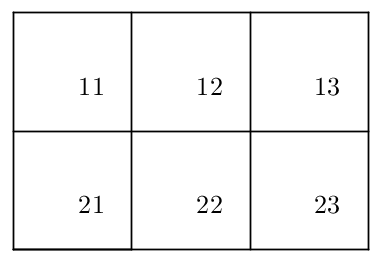
\includegraphics[width=0.25\textwidth]{6-16}
\end{figure}
\bigskip

\noindent풀이)
전체 경우의 수는 \(6!=720\)이다.

여섯 개의 좌석을 주어진 조건에 맞게 세 조로 분할하는 방법은 다음의 세 가지이다.
\begin{figure}[h!]
\centering
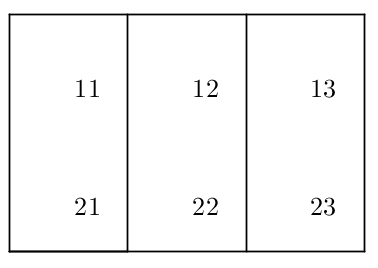
\includegraphics[width=0.25\textwidth]{6-16_1}
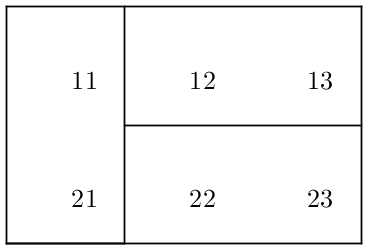
\includegraphics[width=0.25\textwidth]{6-16_2}
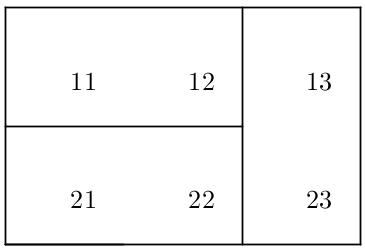
\includegraphics[width=0.25\textwidth]{6-16_3}
\end{figure}
세 조 중 하나를 택하고(\(_3C_1\)), 각 조에 들어갈 학생의 국적을 정하고(\(3!\)), 각 국적의 학생들이 자리에 앉는 방법을 정하면(\((2!)^3\)) 되므로 총 \(144\)가지이다.

따라서 주어진 조건을 만족할 확률은
\(\frac{144}{720}=\frac15\)
이다.

%
\prob{6-17}
주머니에 1부터 9까지의 자연수가 한 개씩 적혀 있는 9개의 공이 들어있다.
이 주머니에서 임의로 3개의 공을 동시에 꺼낼 때, 꺼낸 공에 적혀 있는 수의 합이 홀수이고, 곱이 3의 배수일 확률을 구하여라.
\bigskip

\noindent풀이) 전체 경우의 수는 \(_9C_3=84\)이다.
\(A\)를 세 수의 합이 홀수인 사건, \(B\)를 세 수의 곱이 3의 배수인 사건이라고 하자.
이제 구해야 하는 것은 \(n(A\cap B)\)이다.
이때
\[n(A\cap B)=n(A)-n(A-B)=n(A)-n(A\cap B^c)\]
를 이용하자.

\(n(A)\)를 구하자. 세 수의 합이 홀수인 경우의 수를 구해야 하므로, 주어진 집합 \{1,2,3,4,5,6,7,8,9\}을 짝수들의 집합 \{2,4,6,8\}과 \(\{1,3,5,7,9\}\)로 나누어 생각하자.
세 수의 합이 홀수이려면 (1) 세 수가 모두 홀수이거나, (2) 두 수가 짝수이고 한 수가 홀수이면 된다.
따라서 \(n(A)=_5C_3+_4C_2\times_5C_1=40\)이다.

\(n(A\cap B^c)\)를 구하자.
주어진 \(A\)에서, 곱이 3의 배수가 아닌 경우의 수를 구하면 된다.
따라서 세 수 중에 하나도 3의 배수가 없으면 된다.
그러므로 3의 배수를 제외하여 만든 짝수집합 \{2,4,8\}과 홀수집합 \(\{1,5,7\}\)을 생각하자.
이전과 마찬가지로, 세 수의 합이 홀수이려면 (1) 세 수가 모두 홀수이거나, (2) 두 수가 짝수이고 한 수가 홀수이면 된다.
따라서 \(n(A\cap B^c)=_3C_3+_3C_2\times_3C_1=10\)이다.

따라서 \(n(A\cap B)=40-10=30\)이고
\[
P(A\cap B)=\frac{n(A\cap B)}{n(U)}=\frac{30}{84}=\frac5{14}
\]
이다.

%
\prob{6-20}
정팔각형의 8개의 꼭짓점 중에서 임의로 3개를 잡아 삼각형을 만들 때, 직각삼각형이 될 확률은?

\bigskip
\noindent풀이) 정팔각형에 외접하는 외접원을 생각하자.
직각삼각형이 만들어지려면, 외접원의 지름을 하나 포함해야 한다.
외접원의 지름은 4개를 선택할 수 있고, 외접원을 선택했을 때 나머지 한 점은 6개를 선택할 수 있다.
따라서 구하는 확률은
\[\frac{4\times 6}{_8C_3}=\frac37\]
이다.

%
\prob{6-22}
\(0\le b\le a\le 4\)를 만족하는 두 실수 \(a\), \(b\)를 임의로 택하여 \(x\)에 관한 이차방정식을 만들 때, 이 이차방정식이 실근을 가질 확률을 구하여라.
\bigskip

\noindent풀이)
가능한 \((a,b)\)를 \(a-b\)평면 위에 나타내면 다음과 같은 직각삼각형이 되고, 그 안에서 이차방정식의 판별식이 0보다 크거나 같은 범위가 되는 \(b\ge\frac14a^2\)을 나타내면 다음과 같이 포물선 아래의 영역이 된다.
\begin{figure}[h!]
\centering
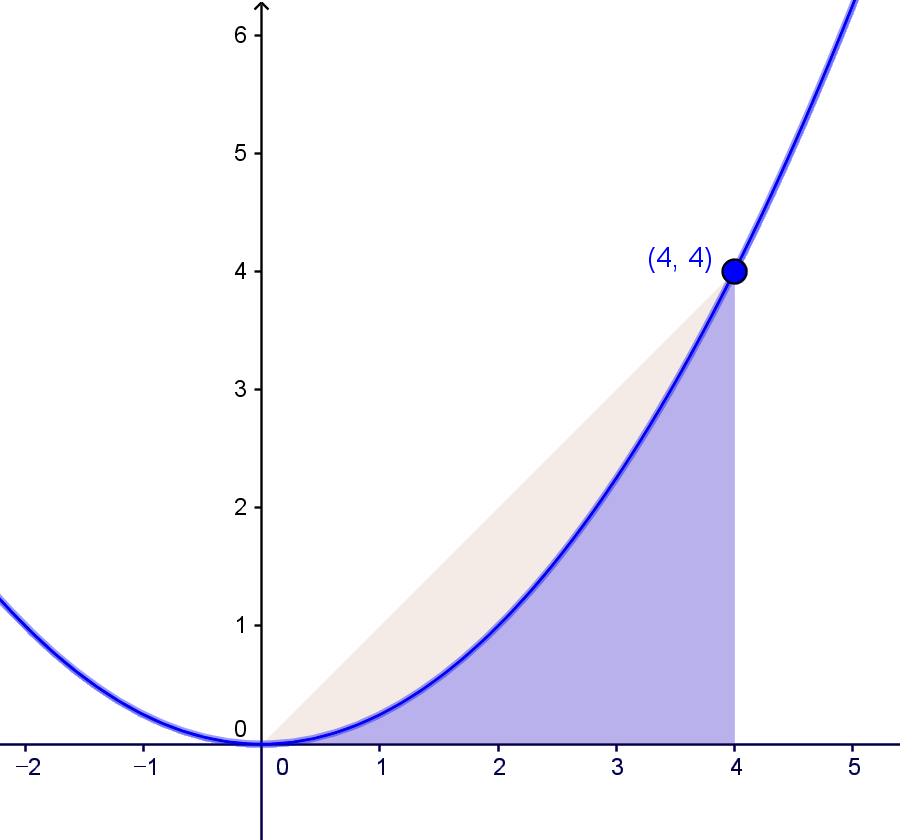
\includegraphics[width=0.4\textwidth]{6-22}
\end{figure}

따라서 구하는 확률은
\[
\frac{\int_0^4\frac14a^2\,da}{\frac12\times 4\times 4}=\frac23
\]
이다.

\newpage
%%
\section{유사 문제들}

%
\prob{6-16-1}
다음과 같이 생긴 2층짜리 아파트가 있다.
여기에 \(A\), \(B\), \(C\), \(D\) 네 개 세대가 입주하는데 \(A\)와 \(B\), \(C\)와 \(D\)는 서로 친척간이다.
친척끼리는 호수의 차가 1또는 100이 되도록 입주할 확률은?
\begin{figure}[h!]
\centering
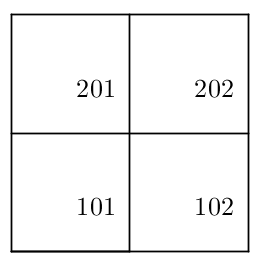
\includegraphics[width=0.25\textwidth]{6-16-1}
\end{figure}

%
\prob{6-16-2}
국어국문학과, 철학과, 심리학과, 사회학과 학생이 각각 두 명씩 있다.
이 학생들이 다음과 같은 열람실의 \(A\)구역의 여덟 좌석에 앉으려고 한다.
같은 학과의 학생끼리는 좌석번호의 차가 1이거나 합이 21이 되도록 앉게 될 확률은?
\begin{figure}[h!]
\centering
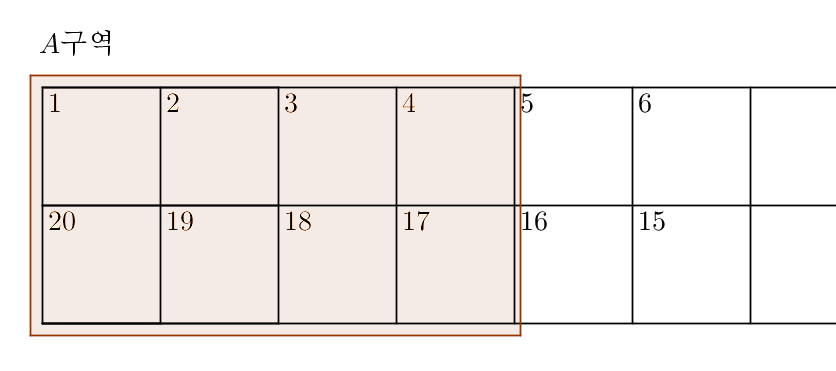
\includegraphics[width=0.7\textwidth]{6-16-2}
\end{figure}

%
\prob{6-17-1}
1부터 12까지의 자연수 중 임의로 두 개를 동시에 선택할 때, 두 수의 합이 짝수일 확률과 두 수의 곱이 짝수일 확률을 각각 구하시오.

%
\prob{6-17-2}
1부터 12까지의 자연수 중 임의로 두 개를 동시에 선택할 때, 두 수의 합이 3의 배수일 확률과 두 수의 곱이 3의 배수일 확률을 각각 구하시오.

%
\prob{6-17-3}
1부터 12까지의 자연수 중 임의로 \textbf{세} 개를 동시에 선택할 때, \textbf{세} 수의 합이 3의 배수일 확률을 구하시오.

%
\prob{6-17-4}
1부터 12까지의 자연수 중 임의로 두 개를 동시에 선택할 때, 두 수의 합이 4의 배수일 확률을 구하시오.

%
\prob{6-20-1}
정육각형의 6개의 꼭짓점 중에서 임의로 3개를 잡아 삼각형을 만들 때, 직각삼각형이 될 확률은?

%
\prob{6-20-2}
정십각형의 10개의 꼭짓점 중에서 임의로 3개를 잡아 삼각형을 만들 때, 직각삼각형이 될 확률은?

%
\prob{6-22-1}
\(0\le a\le 1\), \(0\le b\le 1\)를 만족시키는 두 실수 \(a\), \(b\)를 택해, \(x\)에 관한 이차방정식 \(x^2+ax+b=0\)를 만들 때 이 이차방정식이 실근을 가질 확률은?

%
\prob{6-22-2}
\(0\le b\le 2a\le 12\)를 만족시키는 두 실수 \(a\), \(b\)를 택해, 함수 \(f(x)=x^3+ax^2+bx+10\)을 만들 때 이 함수가 극값을 가질 확률은?

\end{document}